\documentclass{beamer}
\mode<presentation>
{ \usetheme{boxes} }

\usepackage{times}
\usepackage{acronym}
\usepackage{graphicx}
\usepackage[backend=bibtex]{biblatex}

\newcommand{\etal}{\textit{et al}. }
\newcommand{\ie}{\textit{i}.\textit{e}., }
\newcommand{\eg}{\textit{e}.\textit{g}. }
\newcommand{\etc}{\textit{etc}. }

\title{Variability and Transformations}
\author{Marco Craveiro}
\date{\today}

\AtBeginSection[]
{
  \begin{frame}<beamer>
    \frametitle{Outline}
    \tableofcontents[currentsection]
  \end{frame}
}

\bibliography{variability_and_transformations}

\begin{document}

\begin{frame}
\titlepage
v${DOGEN_VERSION}
\end{frame}

\section{Background}

\begin{frame}
\frametitle{What is \ac{MDE}}

\begin{itemize}
\item The previous presentation provided an overview of what \ac{MDE}
  is and why you should consider it for Software Engineering.

\pause

\item \ac{MDE} is a ``development paradigm that uses models as the
  primary artifact of the development process. Usually [\ldots] the
  implementation is (semi-)automatically generated from the
  models.''\cite{brambilla2012model}

\pause

\item \ac{MDE} ``goes beyond the pure development activities and
  encompasses other model-based tasks of a complete software
  engineering process (\eg the model-based evolution of the system or
  the model-driven reverse engineering of a legacy
  system.)''\cite{brambilla2012model}

\pause

\item ``Fundamental'' \ac{MDE} equation: Models + Transformations =
  Software

\end{itemize}

\end{frame}

\begin{frame}
\frametitle{\ac{MDE} Key Components: Models}

\begin{itemize}

\item \ac{MDE} is only interested in a special class of models: those
  which are described according to a \textbf{formal language} and thus
  have precise semantics.

\pause

\item Formal models are written using a \acf{DSL}. The \ac{DSL} is
  designed specifically for modeling.

\pause

\item
  \acf{UML} is an example of such a \ac{DSL}. \ac{UML} has a graphical
  representation~--- called a \emph{concrete syntax}~--- but it also
  has an \emph{abstract syntax}.

\pause

\item A \emph{meta-model} is made up of the abstract syntax and the
  static semantics of the \ac{DSL}. The metamodel is the basis for
  \emph{transformations}.

\end{itemize}

\end{frame}

\begin{frame}
\frametitle{\ac{MDE} Key Components: Transforms}

\begin{itemize}
\item \emph{Transformations}~--- or just transforms~--- can be thought
  of as functions that take models as inputs and produce an output.

\pause

\item We can classify transforms based on the \emph{type} of its
  output:

\pause

\begin{itemize}

\item \textbf{\acf{M2M}}: the output is another model. Note that the
  output can \emph{conform} to the same metamodel or to a different
  metamodel.

\pause

\item \textbf{\acf{M2T}}: the output is a textual representation of
  the model.

\end{itemize}

\pause

\item \ac{M2T} transforms are commonly referred to as
  \emph{generators} because they are a generalisation of the notion of
  a \emph{code generator}.

\end{itemize}

\end{frame}

\section{Variability}

\begin{frame}
\frametitle{Software Product Lines}

\begin{itemize}

\item \ac{MDE} ``pursues the goal of creating a software
  \emph{product} in part or in the whole through one or more
  transformations.''\cite{volter2013model}

\pause

\item Once you have a product, the next logical think is to think of
  \emph{product families}: ``the set of all products that can be
  created with a certain domain architecture is commonly referred to
  as a \emph{software system family}.''\cite{volter2013model}

\pause

\item ``Software product line engineering aims to reduce development
  time, effort, cost, and complexity by taking advantage of the
  commonality within a portfolio of similar
  products.''\cite{voelter2007handling}

\end{itemize}

\end{frame}

\begin{frame}
\frametitle{Software Product Lines}

\begin{itemize}

\item ``The main idea of software product lines is to design a family
  of systems instead of one single system. A family of systems defines
  a set of systems that share substantial commonalities but also
  exhibit explicit variations.''\cite{brambilla2012model}

\pause

\item In theory, \ac{PLE} integrates well with \ac{MDE}: it provides
  an analytical framework with which to model the domain looking for
  variations.

\pause

\item If all went according to plan, we should be able to ``simply''
  supply additional inputs to our models; these then determine the
  \emph{concrete} product we want to produce from the universe of
  \emph{possible} products supported by our models. The key here is
  \emph{variability} and how to express it.

\end{itemize}

\end{frame}

\begin{frame}
\frametitle{Software Product Lines: Variability}

\begin{itemize}

\item ``Variability management is the activity concerned with
  identifying, designing, implementing, and tracing flexibility in
  software product lines (SPLs).''

\pause

\item In practice, there are problems integrating \ac{MDE} with
  \ac{PLE}: ``One of the most interesting question [sic] when it comes
  to software product lines and model driven engineering is how to
  formulate the knowledge of a software product line by using
  models. Especially, the variability aspect is in this context of
  main interest as modeling languages are quite often lacking
  variability as a first-class language
  concept.''\cite{brambilla2012model}

\end{itemize}

\end{frame}

\begin{frame}
\frametitle{Software Product Lines: Variability}

Variability has been around for a long time, in various guises.

\begin{figure}
  \centering
  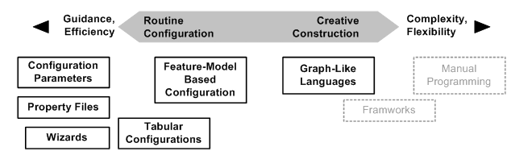
\includegraphics[scale=0.6]{images/variability_spectrum_voelter.png}
  \caption{Expressive power of \ac{DSL}s.\cite{groher2007expressing}}
\end{figure}

\end{frame}

\begin{frame}
\frametitle{Acronyms}

\begin{acronym}
  \acro{DSL}{Domain Specific Language}
  \acro{GPML}{General Purpose Modeling Languages}
  \acro{M2M}{Model-to-Model}
  \acro{M2T}{Model-to-Text}
  \acro{MDE}{Model-driven Engineering}
  \acro{PIM}{Platform Independent Model}
  \acro{PLE}{Product Line Engineering}
  \acro{PSM}{Platform Specific Model}
  \acro{T2M}{Text-to-Model}
  \acro{UML}{Unified Modeling Language}
\end{acronym}

\end{frame}

\begin{frame}
\frametitle{Bibliography}

\printbibliography

\end{frame}



\end{document}
